\documentclass[11pt,twoside]{article}
\usepackage[margin=1in]{geometry}
\usepackage[T1]{fontenc}
\usepackage[nott,notextcomp]{kpfonts}
\usepackage{graphicx}
\usepackage{fancyhdr}
\usepackage{lastpage}

\newcommand{\inlinecode}{\texttt}

% Page layout: stretch text to fill up page.
\addtolength\footskip{.25\headheight}
\flushbottom

% Headings.
\pagestyle{fancy}
\let\headrule\empty
\let\footrule\empty
\lhead{\scshape CSC\,469}
\chead{\large\scshape Assignment \#\,1}
\rhead{\scshape Fall 2016}
\cfoot{\scshape page \thepage\space of \pageref{LastPage}}

\begin{document}
\title{CSC469 A1: Benchmarking}
\author{\textsc{Cheung}, Eugene Yue-Hin (cheun550) and \textsc{Snyder}, Eric (snyderer)}
\date{2016-10-14}
\maketitle


\section{Introduction}
The performance of computer processes can be affected by many greatly varying factors. In this assignment, we performed experiments to explore the sources of interference when a process of interest is running, along with the effects of non-uniform memory access (NUMA) on memory performance. We performed our tests on the Computer Science Teaching Labs's wolf server (\inlinecode{wolf.teach.cs.toronto.edu}), which is currently running Linux 4.4.0-36-generic x86\_64. The following table details some relevant specifications of the server as gathered from \inlinecode{/proc/cpuinfo}, \inlinecode{/proc/meminfo}, \inlinecode{lscpu}, and \inlinecode{GETCONF}:

\begin{table}[!htbp]
    \centering
    \renewcommand{\arraystretch}{1.2}
    \begin{tabular}{|l|l|}
    \hline
    \textbf{CPUs} & 4 $\times$ AMD Opteron 6348 2.8 GHz 12-Core G34 Processor \\
    \hline
    \textbf{CPU cache size} & 2048 KB \\
    \hline
    \textbf{CPU TLB size} & 1536 4K pages \\
    \hline
    \textbf{L1d cache} & 16K \\
    \hline
    \textbf{L1i cache} & 64K \\
    \hline
    \textbf{L2 cache} & 2048K \\
    \hline
    \textbf{L3 cache} & 6144K \\
    \hline
    \textbf{NUMA nodes} & 4 \\
    \hline
    \textbf{NUMA node0 CPUs} & 0-11 \\
    \hline
    \textbf{NUMA node2 CPUs} & 12-23 \\
    \hline
    \textbf{NUMA node4 CPUs} & 24-35 \\
    \hline
    \textbf{NUMA node6 CPUs} & 36-47 \\
    \hline
    \textbf{Total memory} & 65951744 kB \\
    \hline
    \textbf{PAGESIZE} & 4096 kB \\
    \hline
    \end{tabular}
\end{table}


\section{Part A: Process Interference}
To explore the timer interrupt and context switch performance of a Linux system, we developed a tool to measure the performance of several basic operations on x86 systems.


\subsection{Tracking progress activity}

With what frequency do timer interrupts occur?

How long does it take to handle a timer interrupt?

If it appears that there are other, non-timer interrupts (that is, other short periods of inactivity that don't fit the pattern of the periodic timer interrupt), explain what these are likely to be, based on what you can determine about other activity on the system you are measuring.

Over the period of time that the process is running (that is, without lengthy interruptions corresponding to a switch to another process), what percentage of time is lost to servicing interrupts (of any kind)?

\begin{figure}
    \centering
    \includegraphics[width=\textwidth]{parta_activity}
    \caption{Active/inactive periods.}
    \label{fig:activity}
\end{figure}


\subsection{Context switches}
We then attempt to measure the context switch time.

How long is a time slice? 

That is, how long does one process get to run before it is forced to switch to another process? 

Is the length of the time slice affected by the number of processes that you are using? 

Are you surprised by your measurements? 

How does it compare to what you were told about time slices in your previous OS course?

\begin{figure}
    \centering
    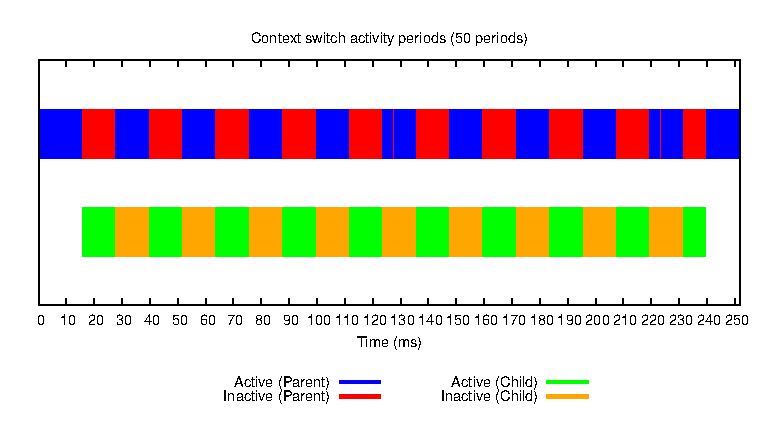
\includegraphics[width=\textwidth]{parta_context}
    \caption{Active/inactive periods for parent/child processes.}
    \label{fig:context}
\end{figure}


\section{Part B: Measuring NUMA Effects}
To explore the effects of the hardware memory organisation on application performance, we specifically measured the effects of NUMA on the performance of standard memory benchmarks. It was expected that memory access from within a node would perform the fastest, while accessing remote memory (i.e. memory in a different node) would result in higher latencies.

\subsection{Methodology}
To test the effects of NUMA time, we ran our experiments on the wolf server as well which uses four interconnected AMD processors with the Magny-Cours architecture. Within a Python 2 script (\inlinecode{partb\_data}), a subprocess was spanwed where \inlinecode{numactl} was executed with the provided precompiled \inlinecode{mccalpin-stream} binary as the command. \inlinecode{numactl} was called with the \inlinecode{membind} argument always set to \inlinecode{0} while the \inlinecode{physcpubind} argument varied. The test was run sequentially four times, choosing a random core from each of the four nodes. Each test was also preceded by a call to \inlinecode{numactl -{}-hardware} to record the free memory available at the time, although this data was left unused. The results then parsed and outputted to a CSV (comma-separated values) file. Table \ref{table:data} shows a sample of the collected data -- the results from the first run, to be specific. To save space, the columns for nodes 2/4/6's free space and the results for the scale, add, and triad tests are not omitted from these results.

\begin{table}[!htbp]
    \centering
    \renewcommand{\arraystretch}{1.2}
    \begin{tabular}{|l|l|l|l|l|l|l|}
    \hline
    \textbf{CPU} & \textbf{Time}    & \textbf{N0 Free} & \textbf{Copy: Best} & \textbf{Copy: Avg} & \textbf{Copy: Min} & \textbf{Copy: Max} \\ \hline
    8            & 1476115806.0167  & 3843             & 4683.1              & 0.090395           & 0.085414           & 0.097353           \\ \hline
    13           & 1476115813.39232 & 3852             & 2928.7              & 0.136969           & 0.136581           & 0.137167           \\ \hline
    24           & 1476115818.81704 & 3852             & 4122.7              & 0.097143           & 0.097024           & 0.097264           \\ \hline
    45           & 1476115824.95741 & 3852             & 3504.6              & 0.114516           & 0.114136           & 0.115149           \\ \hline
    \end{tabular}
    \caption{Sample of collected data.}
    \label{table:data}
\end{table}

The resulting CSV file was later parsed with a second Python 2 script (\inlinecode{partb\_plot}) to generate a bar graph of core occurrences to ensure roughly equal distribution (see Figure \ref{fig:cores}) and a boxplot graph of the four nodes' bandwidth timings (see Figure \ref{fig:nodes}). The four best times from the results of the \inlinecode{mccalpin-stream} program (for the copy, scale, add, and triad tests) were averaged and used as the data points in the boxplot to provide a rough sense of what bandwidths were achieved in the tests. Using a boxplot, we are able to easily see the quartiles and outliers. The graphs were generated using \inlinecode{gnuplot}. Boxplots were generated with \inlinecode{gnuplot}'s default settings (i.e. its default statistical calculations).

In this experiment, the test script was run 256 times over a period of approximately 24 hours. Aside from the first couple of test that were run at sporadic intervals (while setting up the cron job to repeat the test), tests were run every 5 minutes. This resulted in a total of 1,024 rows of data. We can see in Figure \ref{fig:cores} that all 48 of the available cores on the CS Teaching Lab server (cores 0 through 47) were sampled from multiple times at a relatively even distribution. It should also be noted that while the first script to gather data was run on the Teaching Lab server (with Python version 2.7.5), the script to generate the graphs were run on a local machine with macOS 10.12, Python version 2.7.10, and gnuplot version 5.0 patchlevel 4.


\subsection{Results}

\begin{figure}
    \centering
    \includegraphics[width=0.75\textwidth]{partb_cpus}
    \caption{Occurrences of the randomly selected cores in the tests.}
    \label{fig:cores}
\end{figure}

\begin{figure}
    \centering
    \includegraphics[width=0.75\textwidth]{partb_nodes_best}
    \caption{Bandwidth of memory access from the different nodes.}
    \label{fig:nodes}
\end{figure}

The aggregated results from the 256 tests can be seen in Figure \ref{fig:nodes}. The raw data was not filtered in order to achieve as accurate of a graph as possible. As such, outliers can be seen in the graph for nodes 0, 4, and 6, which can likely be explained by higher server load during those tests resulting in lower bandwidths achieved. As expected, memory accesses from node 0 were the fastest (i.e. accessing local memory has lower latency than accessing remote memory). Although the other three nodes were slower, we can see that nodes 4 and 6 performed similarly, while node 2 performed the slowest.

\begin{figure}
    \centering
    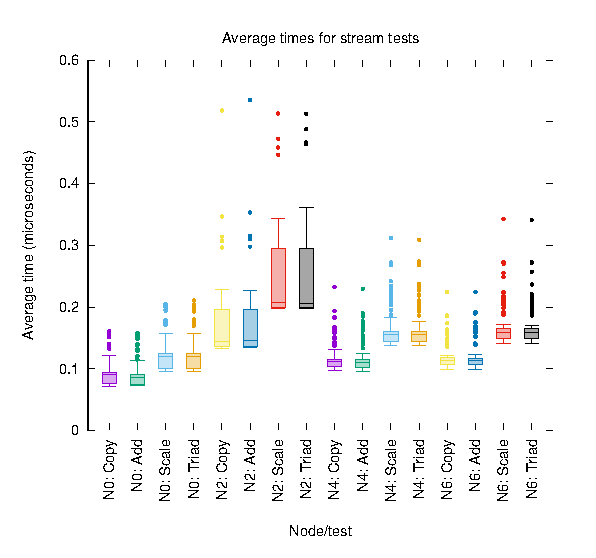
\includegraphics[width=0.8\textwidth]{partb_nodes_avgs}
    \caption{Average test times.}
    \label{fig:nodes_avgs}
\end{figure}

Figure \ref{fig:nodes_avgs} offers more insight into the average timings for the various tests run by \inlinecode{mccalpin-stream} on each node. This corresponds with what we see in Figure \ref{fig:nodes}, where Node 0 performed the fastest (with times hovering around the 0.1$\mu$s mark) and Node 2 performing the worst (with times ranging from around 0.15$\mu$s to 0.2$\mu$s). Like in Figure \ref{fig:nodes}, Nodes 4 and 6 have similar results, with times ranging from around 0.1$\mu$s to 0.15$\mu$s.


\subsection{Discussion}
Interestingly, the results do not seem consistent with the matrix of node distances in the hardware configuration reported by \inlinecode{numactl -{}-hardware}. The reported hardware configuration suggests that all external nodes would perform similarly. On the other hand, the architectural diagram of the Magny-Cours (see Figure \ref{fig:magny}) suggests that one of the nodes (node 3 in the figure) could potentially perform slower due to a higher propagation delay as a result of the physically larger distance. This could be further investigated by running additional tests against different memory nodes to see if a similar pattern appears. From the relatively large amount of outliers seen between Figures \ref{fig:nodes} and \ref{fig:nodes_avgs}, it's likely that clearer results could be achieved during lower/more consistent server load.

\begin{figure}[!htbp]
    \centering
    \includegraphics[width=0.55\textwidth]{Magny-cours-21.png}
    \caption{Architectural diagram of Magny-Cours.}
    \label{fig:magny}
\end{figure}

\end{document}